\chapter{Kromatin dan Epigenetika}\label{ch:b3:chromatin-epigenetics}

Dua ekor mencit dari satu kelahiran, identik secara genetik sampai ke basa
terakhirnya, duduk berdampingan: yang satu ramping dan cokelat, yang lain
gemuk dan kuning, dan kelak akan menderita diabetes. Seekor kucing belang
tiga berbercak jingga dan hitam walaupun setiap sel kulitnya membawa dua
kromosom X yang sama. Seorang anak mewarisi potongan kromosom 15 yang
terhapus, persis seperti anak yang lain, namun yang satu mengidap sindrom
Prader--Willi sedangkan yang lain sindrom Angelman --- bedanya hanya pada
tetua mana yang mewariskan penghapusan itu. Tak satu pun hal ini tertulis di
dalam urutan DNA. Semuanya tertulis \emph{pada} urutan itu: pada cara dua
meter DNA dimampatkan ke dalam nukleus bergaris tengah sepuluh mikrometer,
pada gugus kimia kecil yang terpaut pada protein pemampatnya dan pada
sitosinanya sendiri, dan pada permesinan yang menyalin tanda itu dari sebuah
sel kepada sel anaknya. Bab ini membahas lapisan informasi kedua tersebut,
pengusungnya di tingkat molekul, dan batas jujur dari apa yang sanggup
diingatnya.

\section{Kromatin: DNA pada sebuah kumparan}

\begin{definition}[Nukleosom dan kromatin]\label{def:b3:chromatin-epigenetics:nucleosome}
\index{nukleosom}\index{kromatin}\index{histon}\index{eukromatin}\index{heterokromatin}
Yang disebut \emph{kromatin} adalah kompleks DNA dengan protein, yaitu wujud
keberadaan genom di dalam nukleus eukariot. Satuan berulangnya adalah
\emph{nukleosom}: \qty{147}{bp} DNA yang terlilit $1.65$ putaran kidal
mengelilingi oktamer \emph{histon} --- masing-masing dua salinan protein
kecil yang sangat basa H2A, H2B, H3, dan H4 --- lalu disusul sebuah
\emph{penghubung} sepanjang \qtyrange{20}{60}{bp} menuju nukleosom
berikutnya. Histon kelima, H1, mengikat penghubung itu di tempat DNA masuk
dan meninggalkan intinya, serta membantu manik-manik itu berimpit satu sama
lain. Tiap histon inti mengusung sebuah \emph{ekor} amino-terminal tak
berstruktur sepanjang \numrange{20}{40} residu yang menjulur ke luar
partikel. Kromatin yang terwarnai samar, terkemas longgar, dan ditranskripsi
disebut \emph{eukromatin}; kromatin yang terkemas padat, bereplikasi lambat,
dan sebagian besar bisu --- di sentromer, telomer, dan urutan berulang ---
disebut \emph{heterokromatin}.
\end{definition}

\begin{proof}[Bukti eksperimental]
Hewish dan Burgoyne (1973) mencerna nukleus hati tikus dengan nuklease
endogen dan mendapati DNA-nya keluar bukan sebagai lapisan merata melainkan
sebagai tangga fragmen yang panjangnya kelipatan kira-kira \qty{200}{bp}:
DNA itu terlindungi pada selang yang teratur dan hanya terpotong di
antaranya. Kornberg (1974) menunjukkan bahwa satuan terlindung itu adalah
sebuah partikel berisi delapan \omterm{def:b3:chromatin-epigenetics:nucleosome}{histon} dengan sekitar \qty{200}{bp}, dan
mikrograf elektron \omterm{def:b3:chromatin-epigenetics:nucleosome}{kromatin} yang dibentangkan perlahan memperlihatkan
``manik-manik pada seutas benang''. Luger dan rekan (1997) memecahkan
struktur kristal partikel intinya pada \qty{2.8}{\angstrom}: \qty{147}{bp},
sebuah oktamer dengan ekornya menerobos ke luar di antara lilitan DNA.
\end{proof}

\begin{omfigure}
\begin{tikzpicture}[every node/.style={font=\scriptsize}, >=stealth]
  % beads on a string
  \foreach \x/\y in {0/0, 2.2/0.5, 4.4/0, 6.6/0.5, 8.8/0} {
    \fill[omDef!30] (\x,\y) circle (0.42);
    \draw[very thick, omThm!70!black] (\x,\y) circle (0.5);
  }
  \draw[very thick, omThm!70!black] (-1.1,-0.1) -- (0-0.47,-0.17);
  \draw[very thick, omThm!70!black] (0.47,-0.17) -- (2.2-0.47,0.33);
  \draw[very thick, omThm!70!black] (2.67,0.33) -- (4.4-0.47,-0.17);
  \draw[very thick, omThm!70!black] (4.87,-0.17) -- (6.6-0.47,0.33);
  \draw[very thick, omThm!70!black] (7.07,0.33) -- (8.8-0.47,-0.17);
  \draw[very thick, omThm!70!black] (9.27,-0.17) -- (10.4,-0.1);
  % tails
  \foreach \x/\y in {0/0, 4.4/0, 8.8/0} { \draw[omProp, thick] (\x,\y+0.5) .. controls (\x-0.2,\y+0.9) .. (\x+0.1,\y+1.15); \draw[omProp, thick] (\x,\y-0.5) .. controls (\x+0.2,\y-0.9) .. (\x-0.1,\y-1.15); }
  \foreach \x/\y in {2.2/0.5, 6.6/0.5} { \draw[omProp, thick] (\x,\y+0.5) .. controls (\x-0.2,\y+0.9) .. (\x+0.1,\y+1.15); }
  % H1
  \fill[omMeth!70!black] (1.55,0.05) circle (0.12); \fill[omMeth!70!black] (5.95,0.05) circle (0.12);
  % labels
  \node[above, align=center] at (2.2,1.75) {ekor histon\\(asetilasi, metilasi)};
  \node[below, align=center] at (4.4,-1.35) {partikel inti: oktamer\\$+$ \qty{147}{bp}, $1.65$ putaran};
  \node[below, align=center] at (7.7,-0.55) {DNA penghubung\\\qtyrange{20}{60}{bp}};
  \node[below] at (5.95,-0.1) {H1};
  \draw[<->] (-0.5,-2.2) -- (2.2-0.5,-2.2) node[midway, below] {ulangan $\approx \qty{200}{bp}$, \qty{11}{nm}};
  \draw[gray] (-0.5,-1.95) -- (-0.5,-2.35); \draw[gray] (1.7,-1.95) -- (1.7,-2.35);
\end{tikzpicture}

{\small Serabut \qty{10}{nm}: inti \omterm{def:b3:chromatin-epigenetics:nucleosome}{nukleosom} (biru) pada satu untai DNA
menerus (merah), tiap manik berupa oktamer \omterm{def:b3:chromatin-epigenetics:nucleosome}{histon} dengan ekornya (jingga)
menjulur ke luar, \omterm{def:b3:chromatin-epigenetics:nucleosome}{histon} penghubung H1 (hijau) di titik masuk--keluarnya.
Kira-kira enam \omterm{def:b3:chromatin-epigenetics:nucleosome}{nukleosom} menempati panjang yang diisi \qty{1200}{bp} DNA
telanjang.}
\end{omfigure}

\begin{omfigure}
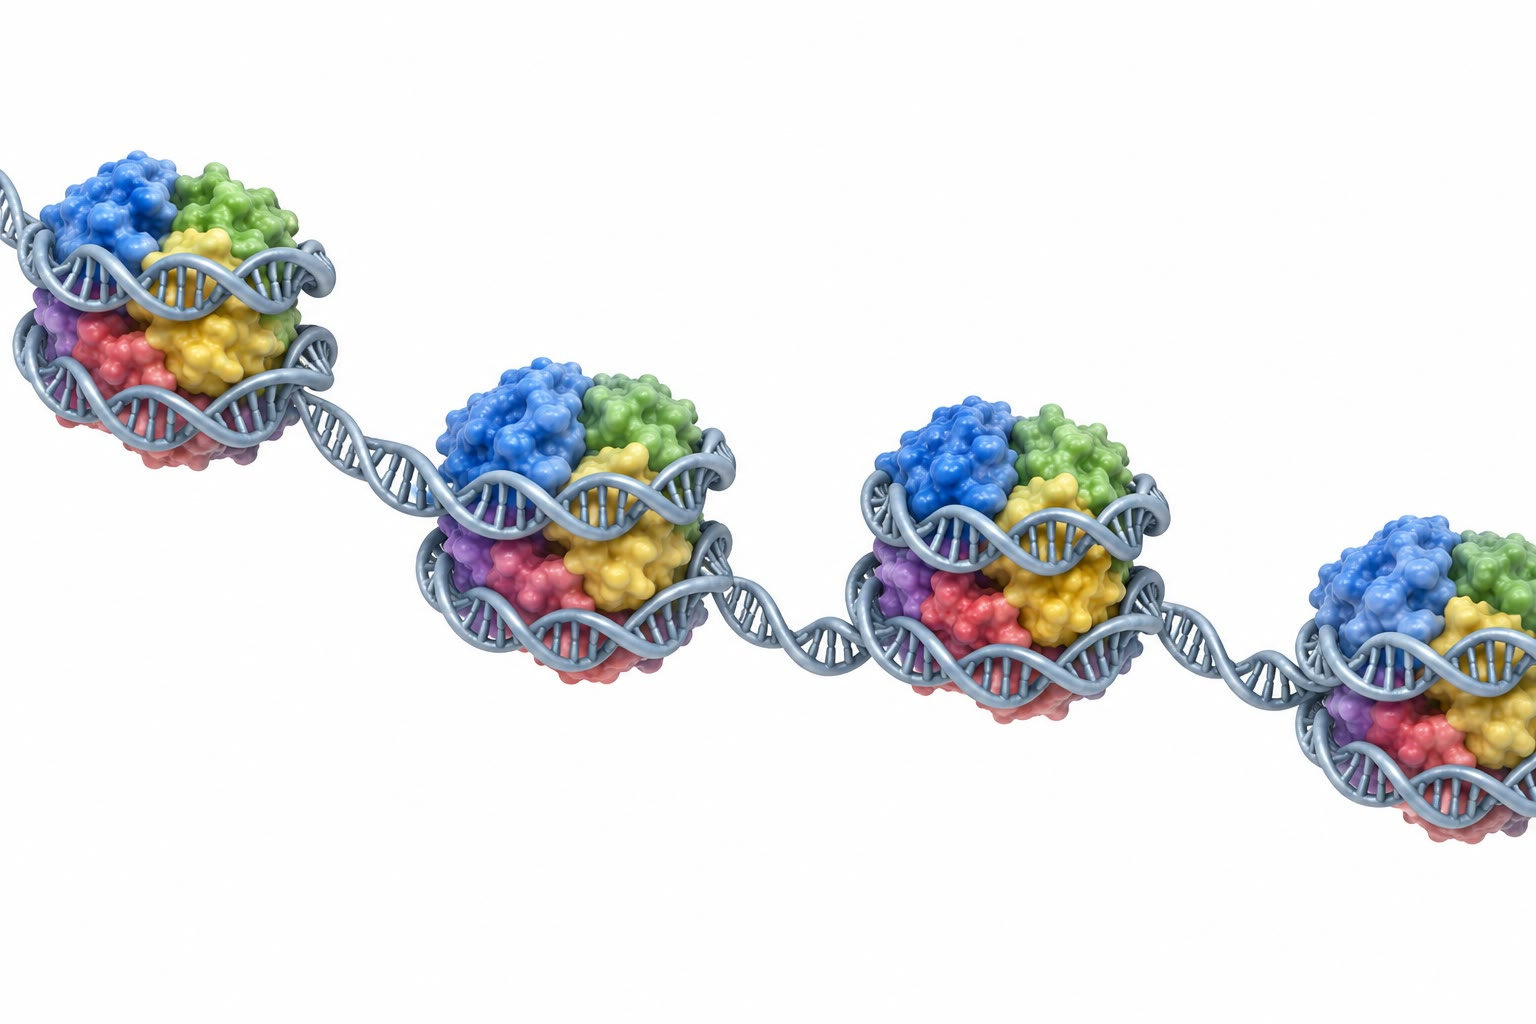
\includegraphics[width=0.6\linewidth]{images/book5/ai/b5-01-nucleosomes.jpg}

{\small \omterm{def:b3:chromatin-epigenetics:nucleosome}{Kromatin} pada skala molekul: heliks ganda yang terlilit pada inti
\omterm{def:b3:chromatin-epigenetics:nucleosome}{histon} berturut-turut, ``manik-manik pada seutas benang'' yang disingkapkan
oleh tangga nuklease itu.}
\end{omfigure}

\begin{proposition}[Tingkat pemampatan]\label{prop:b3:chromatin-epigenetics:compaction}
\index{rasio pemampatan}\index{simpal kromatin}\index{domain terkait topologi}
\emph{\omterm{prop:b3:chromatin-epigenetics:compaction}{Rasio pemampatan}} sebuah struktur \omterm{def:b3:chromatin-epigenetics:nucleosome}{kromatin} adalah panjang DNA yang
dikandungnya dibagi panjang strukturnya. Pelilitan menjadi serabut
\qty{10}{nm} memberi rasio sekitar $6$: \qty{68}{nm} dari satu ulangan
\qty{200}{bp} tertekan menjadi satu manik \qty{11}{nm}. Di dalam nukleus
interfase serabut itu tidak tergulung menjadi serabut tebal yang teratur,
seperti lama digambarkan buku teks, melainkan terlipat menjadi \emph{simpal}
sepanjang puluhan sampai ratusan kilobasa yang tertambat pada pangkalnya oleh
kompleks kohesin berbentuk cincin dan oleh protein pengikat DNA bernama CTCF;
simpal-simpal itu mengelompok menjadi \emph{\omterm{prop:b3:chromatin-epigenetics:compaction}{domain terkait topologi}} (TAD)
sebesar kira-kira satu megabasa, dan di dalamnya sebuah gen jauh lebih sering
berjumpa dengan pengaturnya daripada dengan apa pun di luarnya. Kromosom
mitosis, keadaan yang paling mampat, memiliki \omterm{prop:b3:chromatin-epigenetics:compaction}{rasio pemampatan} mendekati
\num{10000}: \qty{4}{cm} DNA sebuah kromosom manusia rata-rata terlipat
menjadi batang sepanjang \qty{4}{\micro m}.
\end{proposition}

\begin{example}[Dua meter di dalam sepuluh mikrometer]\label{ex:b3:chromatin-epigenetics:two-metres}
Sebuah nukleus diploid manusia memuat $6.4\times 10^{9}$ pasangan basa. Pada
\qty{0.34}{nm} tiap pasangan basa itu berarti \qty{2.2}{m} heliks ganda, di
dalam nukleus bergaris tengah kira-kira \qty{10}{\micro m}. Semuanya terkemas
menjadi $6.4\times 10^{9}/200 \approx 3.2\times 10^{7}$ \omterm{def:b3:chromatin-epigenetics:nucleosome}{nukleosom}, dan
masing-masing mengusung sekitar \qty{108}{kDa} \omterm{def:b3:chromatin-epigenetics:nucleosome}{histon} berbanding \qty{96}{kDa}
DNA (\qty{147}{bp} pada \qty{650}{Da} tiap pasangan): nukleus memuat \omterm{def:b3:chromatin-epigenetics:nucleosome}{histon}
kira-kira sebanyak DNA menurut massanya. DNA-nya sendiri, bila diperlakukan
sebagai silinder bergaris tengah \qty{2}{nm}, hanya bervolume sekitar
\qty{7}{\micro m^3}, yaitu sekitar \qty{1}{\%} dari nukleus bola berjari-jari
\qty{5}{\micro m}; masalah pengemasannya adalah masalah kekusutan dan akses,
bukan masalah ruang.
\end{example}

\section{Sandi histon}

\begin{definition}[Modifikasi histon]\label{def:b3:chromatin-epigenetics:histone-code}
\index{sandi histon}\index{asetilasi}\index{metilasi histon}%
\index{penulis}\index{pembaca}\index{penghapus}
Residu ekor \omterm{def:b3:chromatin-epigenetics:nucleosome}{histon} dimodifikasi secara kovalen: \emph{asetilasi} lisina
(yang menetralkan muatan positifnya dan mengendurkan cengkeramannya pada
DNA), \emph{metilasi} lisina dan arginina (satu, dua, atau tiga gugus metil,
tanpa perubahan muatan), fosforilasi serina, ubikuitinasi lisina. Sebuah
modifikasi dinamai menurut \omterm{def:b3:chromatin-epigenetics:nucleosome}{histon}, residu, dan gugusnya: H3K4me3 adalah
\omterm{def:b3:chromatin-epigenetics:nucleosome}{histon} H3, lisina 4, termetilasi tiga kali; H3K27ac adalah H3 lisina 27
terasetilasi. Yang disebut \emph{sandi \omterm{def:b3:chromatin-epigenetics:nucleosome}{histon}} adalah keterkaitan antara
gabungan tanda dan keadaan gen di bawahnya: H3K4me3 dan H3K27ac pada promotor
dan penguat yang aktif, H3K36me3 sepanjang tubuh gen yang ditranskripsi,
H3K9me3 pada \omterm{def:b3:chromatin-epigenetics:nucleosome}{heterokromatin} konstitutif, H3K27me3 pada gen yang dibungkam
selama perkembangan. Enzim yang menambahkan tanda disebut \emph{penulis}
(\omterm{def:b3:chromatin-epigenetics:nucleosome}{histon} asetiltransferase, HAT; metiltransferase), enzim yang membuangnya
disebut \emph{penghapus} (\omterm{def:b3:chromatin-epigenetics:nucleosome}{histon} deasetilase, HDAC; demetilase), dan protein
yang mengikat sebuah tanda lalu bertindak atasnya disebut \emph{pembaca}:
sebuah \emph{bromodomain} mengikat asetil-lisina, sebuah \emph{kromodomain}
mengikat metil-lisina.
\end{definition}

\begin{proposition}[Tanda dibaca, bukan sekadar dirasakan]\label{prop:b3:chromatin-epigenetics:readers}
\index{HP1}\index{Polycomb}\index{PRC2}\index{Trithorax}
\omterm{def:b3:chromatin-epigenetics:histone-code}{Asetilasi} bekerja sebagian lewat elektrostatika --- ekor yang terasetilasi
memegang DNA-nya lebih longgar dan serabutnya membuka --- tetapi sebagian
besar tanda bekerja dengan merekrut \omterm{def:b3:chromatin-epigenetics:histone-code}{pembaca}. H3K9me3 diikat oleh kromodomain
\emph{protein \omterm{def:b3:chromatin-epigenetics:nucleosome}{heterokromatin} HP1}, yang membentuk dimer, menjembatani
\omterm{def:b3:chromatin-epigenetics:nucleosome}{nukleosom} bertetangga, lalu merekrut metiltransferase (SUV39H) yang justru
menuliskan H3K9me3 pada \omterm{def:b3:chromatin-epigenetics:nucleosome}{nukleosom} berikutnya: tandanya merambat sepanjang
serabut sampai bertemu sebuah batas, dan memampatkan apa pun yang
diliputinya. H3K27me3 dituliskan oleh \emph{kompleks represif Polycomb 2}
(PRC2, subunit katalitiknya EZH2), dibaca oleh PRC1, yang mengubikuitinasi
H2A dan memampatkan serabutnya, dan kompleks itu sendiri dirangsang oleh
tanda yang dibuatnya; kelompok protein \emph{Trithorax} menuliskan H3K4me3
yang berlawanan dan menjaga gen perkembangan suatu tipe sel tetap menyala.
Tiap gelung semacam itu --- \omterm{def:b3:chromatin-epigenetics:histone-code}{pembaca} merekrut \omterm{def:b3:chromatin-epigenetics:histone-code}{penulis} --- adalah umpan balik
positif yang memungkinkan sebuah keadaan memelihara dirinya sendiri sesudah
mapan, dan itulah yang dibutuhkan sebuah tanda yang diwariskan.
\end{proposition}

\begin{omfigure}
\begin{tikzpicture}[every node/.style={font=\scriptsize}, >=stealth]
  % nucleosomes with tails
  \foreach \x in {0,2,4,6} { \draw[thick, omDef, fill=omDef!20] (\x,0) circle (0.45); \draw[omProp, thick] (\x,0.45) -- (\x,1.15); }
  % marks
  \fill[omThm] (2,1.15) circle (0.11); \fill[omThm] (4,1.15) circle (0.11);
  \fill[omMeth!80!black] (0,1.15) circle (0.11);
  \node[left] at (-0.5,1.15) {ac};
  \node[right, align=left] at (6.15,1.15) {me3};
  % HP1 reader
  \draw[thick, fill=omExo!30] (2.6,1.7) ellipse (0.5 and 0.25); \node at (2.6,1.7) {pembaca};
  \draw[thick, fill=omExo!30] (4.2,2.35) ellipse (0.55 and 0.25); \node at (4.2,2.35) {penulis};
  \draw[->, thick] (2.9,1.9) -- (3.75,2.2);
  \draw[->, thick, omThm] (4.6,2.15) .. controls (5.6,2.0) and (6.1,1.8) .. (6.05,1.3);
  \node[right, align=left, font=\scriptsize] at (6.6,2.0) {merambat ke\\nukleosom berikutnya};
  \draw[->, thick, gray] (2.2,1.3) -- (2.45,1.5);
  % eraser
  \draw[thick, fill=omExo!30] (0.6,2.2) ellipse (0.5 and 0.25); \node at (0.6,2.2) {penghapus};
  \draw[->, thick, omMeth!80!black] (0.3,2.0) -- (0.05,1.35);
  % DNA
  \draw[very thick, omThm!70!black] (-0.9,-0.3) -- (-0.45,-0.05) (0.45,-0.05) -- (1.55,-0.05) (2.45,-0.05) -- (3.55,-0.05) (4.45,-0.05) -- (5.55,-0.05) (6.45,-0.05) -- (7.2,-0.3);
  \node[below, align=center] at (0,-0.6) {terbuka: gugus asetil\\menghapus satu muatan};
  \node[below, align=center] at (5,-0.6) {tertutup: H3K9me3 dibaca HP1,\\yang merekrut metilase K9};
\end{tikzpicture}

{\small Logika penulis--pembaca--penghapus. Sebuah \omterm{def:b3:chromatin-epigenetics:histone-code}{pembaca} yang terikat pada
tanda di satu \omterm{def:b3:chromatin-epigenetics:nucleosome}{nukleosom} merekrut \omterm{def:b3:chromatin-epigenetics:histone-code}{penulis} yang memasang tanda yang sama pada
\omterm{def:b3:chromatin-epigenetics:nucleosome}{nukleosom} berikutnya, sehingga keadaan itu merambat dan menyalin dirinya
sendiri; \omterm{def:b3:chromatin-epigenetics:histone-code}{penghapus} melawannya. Gugus asetil (hijau) membuka serabutnya;
H3K9me3 (merah) menutupnya.}
\end{omfigure}

\begin{method}[Imunopresipitasi kromatin (ChIP)]\label{met:b3:chromatin-epigenetics:chip}
\index{ChIP}\index{imunopresipitasi kromatin}
Untuk memetakan letak sebuah tanda atau protein pada genom: (1) taut-silangkan
protein pada DNA di dalam sel hidup dengan formaldehida; (2) cacah \omterm{def:b3:chromatin-epigenetics:nucleosome}{kromatinnya}
menjadi fragmen sepanjang beberapa ratus pasangan basa; (3) endapkan
fragmennya dengan antibodi terhadap tanda itu (misalnya H3K27me3) yang terikat
pada butiran; (4) balikkan taut-silangnya lalu murnikan DNA-nya; (5) urutkan
DNA itu (ChIP-seq) dan cacah bacaannya sepanjang genom: puncaknya adalah
tempat tanda itu berada. Kendali berupa DNA masukan tanpa antibodi menetapkan
latarnya. Daya pisahnya sebesar fragmennya, kira-kira satu \omterm{def:b3:chromatin-epigenetics:nucleosome}{nukleosom}.
\end{method}

\begin{remark}[Sandi atau keterkaitan]\label{rem:b3:chromatin-epigenetics:code}
Kata ``sandi'' melebih-lebihkan keadaannya. Banyak tanda merupakan akibat
transkripsi, bukan penyebabnya (H3K36me3 diletakkan oleh metiltransferase yang
membonceng polimerase), dan membuang sebuah \omterm{def:b3:chromatin-epigenetics:histone-code}{penulis} sering mengubah ekspresi
jauh lebih sedikit daripada yang disarankan sebaran tandanya. Yang mapan
adalah bahwa beberapa tanda --- H3K9me3, H3K27me3, dan \omterm{def:b3:chromatin-epigenetics:methylation}{metilasi DNA} di
bawah --- mengusung pembungkaman yang merambat sendiri dan hidup lebih lama
daripada isyarat yang memasangnya.
\end{remark}

\section{Metilasi DNA dan penyalinan sebuah tanda}

\begin{definition}[Metilasi DNA]\label{def:b3:chromatin-epigenetics:methylation}
\index{metilasi DNA}\index{CpG}\index{pulau CpG}%
\index{DNMT1}\index{metilasi pemeliharaan}\index{metilasi de novo}
Pada vertebrata sebuah gugus metil ditambahkan pada karbon 5 sitosina hampir
hanya di dalam dinukleotida \emph{CpG} (sebuah C yang disusul G pada untai
yang sama), yaitu urutan yang menjadi komplemennya sendiri, sehingga CpG yang
termetilasi lazimnya termetilasi pada kedua untainya. Sekitar
\qtyrange{70}{80}{\%} CpG sebuah sel manusia termetilasi, dan promotor yang
termetilasi bersifat bisu: gugus metilnya dibaca oleh protein pengikat
metil-CpG (MeCP2, MBD1--4) yang merekrut HDAC dan metilase H3K9, dan gugus itu
langsung menghalangi beberapa faktor transkripsi. Kekecualiannya adalah
\emph{pulau CpG}, bentangan sepanjang kira-kira satu kilobasa, kaya G dan C
serta kaya CpG, yang duduk pada promotor sebagian besar gen rumah tangga dan
tetap tak termetilasi di dalam sel normal. Gugus metil dituliskan oleh
\emph{metiltransferase DNA}: DNMT3A dan DNMT3B menjalankan \emph{metilasi de
novo} pada tapak yang belum termetilasi, sedangkan \emph{DNMT1}, yang lebih
menyukai CpG hemimetilasi --- satu untai termetilasi, untai lain tidak ---
menjalankan \emph{metilasi pemeliharaan} di belakang garpu replikasi.
Pembuangannya bersifat pasif, lewat replikasi tanpa pemeliharaan, atau aktif,
lewat enzim TET, yang mengoksidasi 5-metilsitosina menjadi
5-hidroksimetilsitosina dan seterusnya sampai perbaikan eksisi basa
menggantinya dengan sitosina biasa.
\end{definition}

\begin{example}[Mengapa genom kekurangan CpG]\label{ex:b3:chromatin-epigenetics:cpg-deficit}
Genom manusia mengandung \qty{42}{\%} G$+$C, sehingga andaikan basanya saling
bebas sebuah \omterm{def:b3:chromatin-epigenetics:methylation}{CpG} akan muncul dengan frekuensi $0.21\times 0.21 \approx 0.044$,
yakni sekitar $2.8\times 10^{8}$ kali di dalam genom diploid. Cacah
teramatinya sekitar $5.6\times 10^{7}$, seperlima dari itu. Sebabnya adalah
tandanya sendiri: sitosina termetilasi yang kehilangan gugus aminonya menjadi
timina, basa normal yang tidak dapat dikenali sebagai salah oleh permesinan
perbaikan, sedangkan sitosina tak termetilasi terdeaminasi menjadi urasil,
yang dieksisi. Sepanjang waktu evolusi \omterm{def:b3:chromatin-epigenetics:methylation}{CpG} yang termetilasi telah bermutasi
menjadi TpG dan CpA, dan hanya pulau yang tak termetilasi yang mempertahankan
\omterm{def:b3:chromatin-epigenetics:methylation}{CpG-nya}. Tanda itu meninggalkan jejaknya di dalam urutan.
\end{example}

\begin{theorem}[Pemeliharaan keadaan metilasi sepanjang pembelahan]\label{thm:b3:chromatin-epigenetics:maintenance}
\index{ingatan epigenetik}\index{rantai Markov!metilasi}
Tinjaulah satu tapak \omterm{def:b3:chromatin-epigenetics:methylation}{CpG}, yang diikuti sepanjang satu garis keturunan sel.
Pada tiap pembelahan sitosina untai baru termetilasi dengan peluang $\mu$
apabila sitosina untai cetakannya termetilasi (daya guna pemeliharaan) dan
dengan peluang $\delta$ apabila tidak (laju de novo). Misalkan $p_{n}$ adalah
peluang tapak itu termetilasi sesudah $n$ pembelahan. Maka
\[
p_{n+1} = \mu\, p_{n} + \delta\,(1 - p_{n}),
\qquad
p_{n} = p^{*} + (p_{0} - p^{*})\,(\mu - \delta)^{n},
\qquad
p^{*} = \frac{\delta}{1 - \mu + \delta}.
\]
Setiap tapak menghanyut menuju kesetimbangan $p^{*}$ yang sama, apa pun
keadaan awalnya, dan ingatan akan keadaan awal itu meluruh secara geometrik
dengan rasio $\mu - \delta$. Sebuah tanda diingat selama kira-kira
$1/(1 - \mu + \delta)$ pembelahan; ingatan yang setia akan \emph{selisih}
antartapak karena itu menuntut $\mu$ sangat dekat ke $1$ dan $\delta$ sangat
dekat ke $0$, atau menuntut umpan balik yang membuat $\mu$ dan $\delta$
bergantung pada keadaan tetangganya.
\end{theorem}
\begin{proof}
Rekurensinya adalah hukum peluang total atas kedua keadaan untai cetakan.
Titik tetapnya memenuhi $p^{*} = \mu p^{*} + \delta(1 -
p^{*})$, sehingga $p^{*}(1 - \mu + \delta) = \delta$. Dengan mengurangkan persamaan titik tetap
itu dari rekurensinya diperoleh $p_{n+1} - p^{*} = (\mu -
\delta)(p_{n} - p^{*})$, yang bila diiterasi memberi bentuk tertutupnya. Karena
$0 \le \delta \le \mu \le 1$, rasio $\mu - \delta$ terletak di $[0,1]$ dan
simpangannya mengecil; simpangan itu separuh setiap $\ln 2 / (-\ln(\mu -
\delta)) \approx \ln 2/(1 - \mu + \delta)$ pembelahan ketika $\mu -
\delta$ dekat ke $1$.
\end{proof}

\begin{example}[Angka-angkanya]\label{ex:b3:chromatin-epigenetics:maintenance-numbers}
Nilai terukur bagi sel mamalia adalah $\mu \approx 0.99$ dan
$\delta \approx 0.02$ tiap pembelahan pada \omterm{def:b3:chromatin-epigenetics:methylation}{CpG} yang lazim. Maka $p^{*} =
0.02/0.03 \approx 0.67$, dekat dengan fraksi termetilasi seluruh genom, dan
$\mu - \delta = 0.97$: tapak yang termetilasi penuh lalu dibiarkan pada
permesinannya saja akan berada separuh jalan kembali ke rata-rata sesudah $\ln 2 /
0.03 \approx 23$ pembelahan. Promotor yang dibungkam dan tetap bisu
selama ratusan pembelahan seumur hidup karena itu menuntut lebih daripada
\omterm{def:b3:chromatin-epigenetics:methylation}{DNMT1}: \omterm{def:b3:chromatin-epigenetics:histone-code}{pembaca} \omterm{def:b3:chromatin-epigenetics:methylation}{metil-CpG} merekrut metilasi H3K9 dan \omterm{def:b3:chromatin-epigenetics:histone-code}{pembaca} H3K9 merekrut
DNMT3, sehingga pulau tanda yang rapat menaikkan $\mu$-nya sendiri menuju $1$
dan menurunkan $\delta$ tetangganya menuju $0$. Sebaliknya, sel yang
kehilangan \omterm{def:b3:chromatin-epigenetics:methylation}{DNMT1} kehilangan tandanya secara pasif: dengan
$\mu = \delta = 0$ fraksi untai yang termetilasi separuh pada tiap
pembelahan.
\end{example}

\begin{omfigure}
\begin{tikzpicture}[every node/.style={font=\scriptsize}, >=stealth]
  % left: replication scheme
  \begin{scope}
    \draw[very thick, omThm!70!black] (0,1.2) -- (2.4,1.2); \draw[very thick, omThm!70!black] (0,0.9) -- (2.4,0.9);
    \foreach \x in {0.5,1.2,1.9} { \fill[omDef] (\x,1.2) circle (0.09); \fill[omDef] (\x,0.9) circle (0.09); }
    \node[above] at (1.2,1.3) {tetua: kedua untai termetilasi};
    \draw[->, thick] (1.2,0.75) -- (1.2,0.15) node[midway, right] {replikasi};
    \draw[very thick, omThm!70!black] (0,-0.1) -- (2.4,-0.1); \draw[very thick, gray] (0,-0.4) -- (2.4,-0.4);
    \foreach \x in {0.5,1.2,1.9} { \fill[omDef] (\x,-0.1) circle (0.09); \draw[omDef] (\x,-0.4) circle (0.09); }
    \node[left] at (-0.1,-0.25) {hemimetilasi};
    \draw[->, thick] (1.2,-0.85) -- (1.2,-1.45) node[midway, right, align=left] {DNMT1, peluang $\mu$\\tiap tapak};
    \draw[very thick, omThm!70!black] (0,-1.7) -- (2.4,-1.7); \draw[very thick, gray] (0,-2.0) -- (2.4,-2.0);
    \foreach \x in {0.5,1.9} { \fill[omDef] (\x,-1.7) circle (0.09); \fill[omDef] (\x,-2.0) circle (0.09); }
    \fill[omDef] (1.2,-1.7) circle (0.09); \draw[omDef] (1.2,-2.0) circle (0.09);
    \node[below, align=center] at (1.2,-2.1) {pulih, satu tapak terlewat:\\untai baru sel anaknya};
  \end{scope}
  % right: decay plot
  \begin{scope}[xshift=5.0cm, yshift=-2.3cm]
  \begin{axis}[
    width=6.6cm, height=4.6cm, axis lines=left,
    xmin=0, xmax=100, ymin=0, ymax=1.05,
    xlabel={pembelahan $n$},
    xlabel style={font=\scriptsize, at={(axis description cs:0.5,-0.1)}, anchor=north},
    tick label style={font=\scriptsize}, xtick={0,25,50,75,100}, ytick={0,0.5,0.67,1},
    yticklabels={0,0.5,$p^{*}$,1}, clip=false,
  ]
  \addplot[very thick, omDef, domain=0:100, samples=60] {0.6667 + 0.3333*0.97^x};
  \addplot[very thick, omThm, domain=0:100, samples=60] {0.6667 - 0.6667*0.97^x};
  \addplot[dashed, gray, domain=0:100, samples=2] {0.6667};
  \addplot[thick, omMeth!80!black, domain=0:100, samples=60] {0.6667 + 0.3333*0.998^x};
  \node[font=\scriptsize] at (axis cs:-9,1.1) {$p_{n}$};
  \node[font=\scriptsize, omDef, anchor=south west] at (axis cs:45,0.82) {awal termetilasi, $\mu = 0.99$};
  \node[font=\scriptsize, omThm, anchor=north west] at (axis cs:50,0.30) {awal tak termetilasi};
  \node[font=\scriptsize, omMeth!80!black, anchor=south west] at (axis cs:30,1.02) {dengan umpan balik, $\mu = 0.999$};
  \end{axis}
  \end{scope}
\end{tikzpicture}

{\small Kiri: \omterm{def:b3:chromatin-epigenetics:methylation}{metilasi pemeliharaan}. Sesudah replikasi setiap \omterm{def:b3:chromatin-epigenetics:methylation}{CpG} bersifat
hemimetilasi; \omterm{def:b3:chromatin-epigenetics:methylation}{DNMT1} menyalin tandanya ke untai baru dengan peluang $\mu$ tiap
tapak. Kanan: nasib sebuah tapak sepanjang pembelahan untuk $\mu = 0.99$,
$\delta = 0.02$ (biru dari keadaan termetilasi, merah dari keadaan tak
termetilasi) --- keduanya memusat ke $p^{*} = 0.67$ --- dan untuk tapak yang
umpan balik tetangganya menaikkan $\mu$ menjadi $0.999$ (hijau).}
\end{omfigure}

\begin{method}[Membaca metilasi: pengurutan bisulfit]\label{met:b3:chromatin-epigenetics:bisulfite}
\index{pengurutan bisulfit}
Pengurutan saja tidak dapat melihat sebuah gugus metil. Perlakukan DNA yang
telah didenaturasi dengan natrium bisulfit: sitosina tak termetilasi
terdeaminasi menjadi urasil, yang terbaca sebagai T sesudah PCR, sedangkan
5-metilsitosina terlindungi dan tetap terbaca sebagai C. Urutkan DNA hasil
konversinya lalu bandingkan dengan acuannya: setiap C yang tetap C tadinya
termetilasi, setiap C yang menjadi T tidak. Bila dikerjakan seluruh genom
(\omterm{met:b3:chromatin-epigenetics:bisulfite}{pengurutan bisulfit} seluruh genom) cara ini memberi keadaan metilasi setiap
dari $2.8\times 10^{7}$ \omterm{def:b3:chromatin-epigenetics:methylation}{CpG} sebuah genom haploid pada daya pisah satu basa,
sebagai fraksi sel di dalam contohnya.
\end{method}

\section{Penonaktifan X dan pencetakan genomik}

\begin{definition}[Penonaktifan kromosom X]\label{def:b3:chromatin-epigenetics:x-inactivation}
\index{penonaktifan X}\index{badan Barr}\index{Xist}\index{kompensasi dosis}
Pada mamalia betina salah satu dari dua kromosom X setiap sel somatik
dibungkam secara transkripsi sejak dini dalam perkembangan, suatu bentuk
\emph{kompensasi dosis} yang menyetarakan ekspresi gen terpaut-X antara betina
XX dan jantan XY. Kromosom yang dibungkam itu dimampatkan menjadi badan padat
yang menempel pada selubung inti, yaitu \emph{badan Barr}. Pilihan X mana yang
dibungkam bersifat acak di dalam embrio sendiri dan, sekali dibuat, diwariskan
secara klonal oleh seluruh keturunan sel itu. Penonaktifannya diprakarsai oleh
\emph{Xist}, RNA tak penyandi sepanjang \qty{17}{kb} yang ditranskripsi dari
pusat penonaktifan-X kromosom yang akan dibungkam: RNA itu menyelimuti
kromosom tersebut secara cis, lalu merekrut Polycomb (H3K27me3), varian
\omterm{def:b3:chromatin-epigenetics:nucleosome}{histon} makroH2A, dan akhirnya \omterm{def:b3:chromatin-epigenetics:methylation}{metilasi DNA} pada promotornya, dan sesudah itu
kebisuannya terpelihara tanpa Xist perlu hadir pada tiap pembelahan. Sekitar
\qty{15}{\%} gen terpaut-X manusia lolos dari penonaktifan, sebagian atau
seluruhnya.
\end{definition}

\begin{proof}[Bukti eksperimental]
Barr dan Bertram (1949) memperhatikan adanya badan padat di dalam nukleus
neuron kucing betina, tetapi tidak pada yang jantan. Ohno (1959) menunjukkan
bahwa badan itu adalah satu kromosom X utuh yang memadat. Lyon (1961)
merangkai keping-kepingnya: mencit betina heterozigot untuk gen warna bulu
terpaut-X memiliki bulu mozaik berbercak yang mengekspresikan alel yang satu
atau yang lain, sehingga tiap bercak adalah satu klon yang salah satu X-nya,
selalu X yang sama, bisu; hal yang sama berlaku bagi bercak jingga dan hitam
kucing belang tiga, yang gen jingganya terpaut-X, dan bagi kelenjar keringat
mozaik perempuan pembawa alel mutan sebuah gen terpaut-X. Kucing belang tiga
jantan hampir selalu XXY.
\end{proof}

\begin{omfigure}
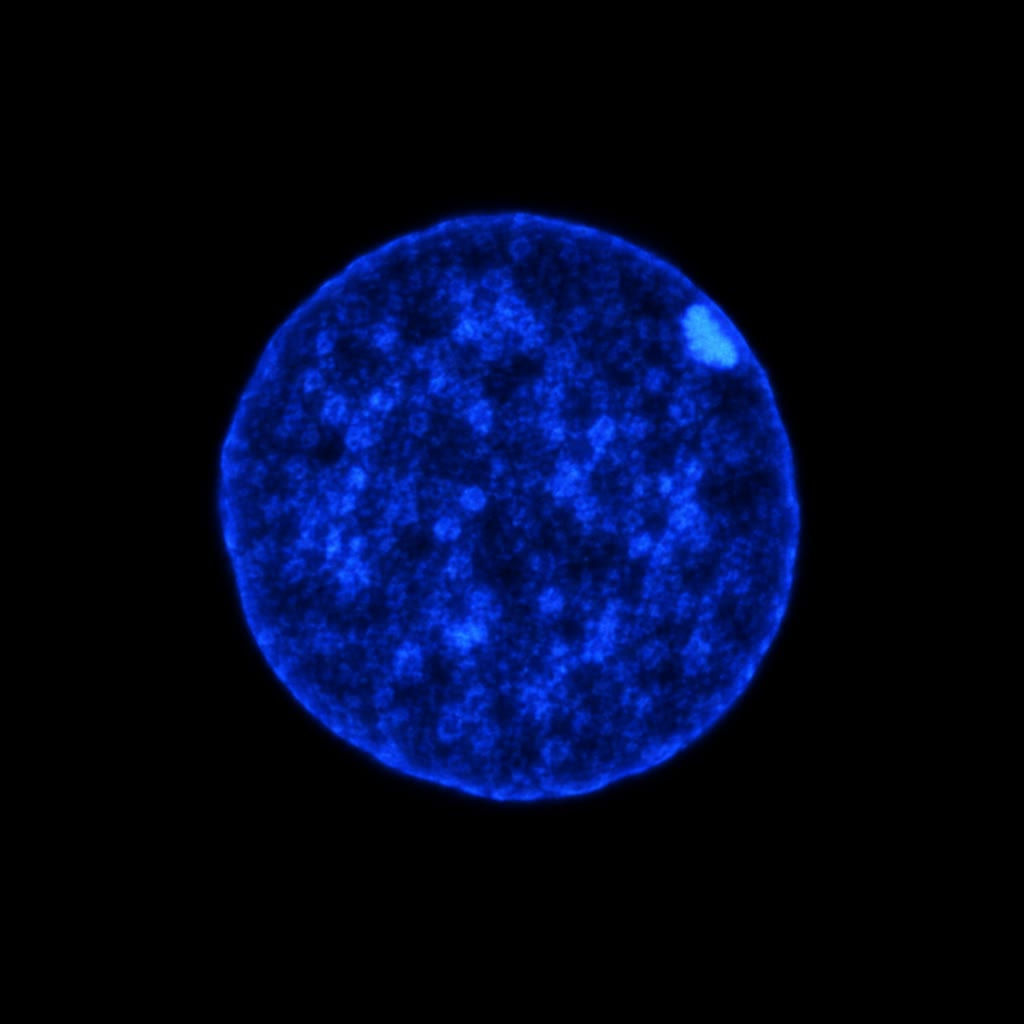
\includegraphics[width=0.42\linewidth]{images/book5/ai/b5-01-barr-body.jpg}\hspace{0.04\linewidth}
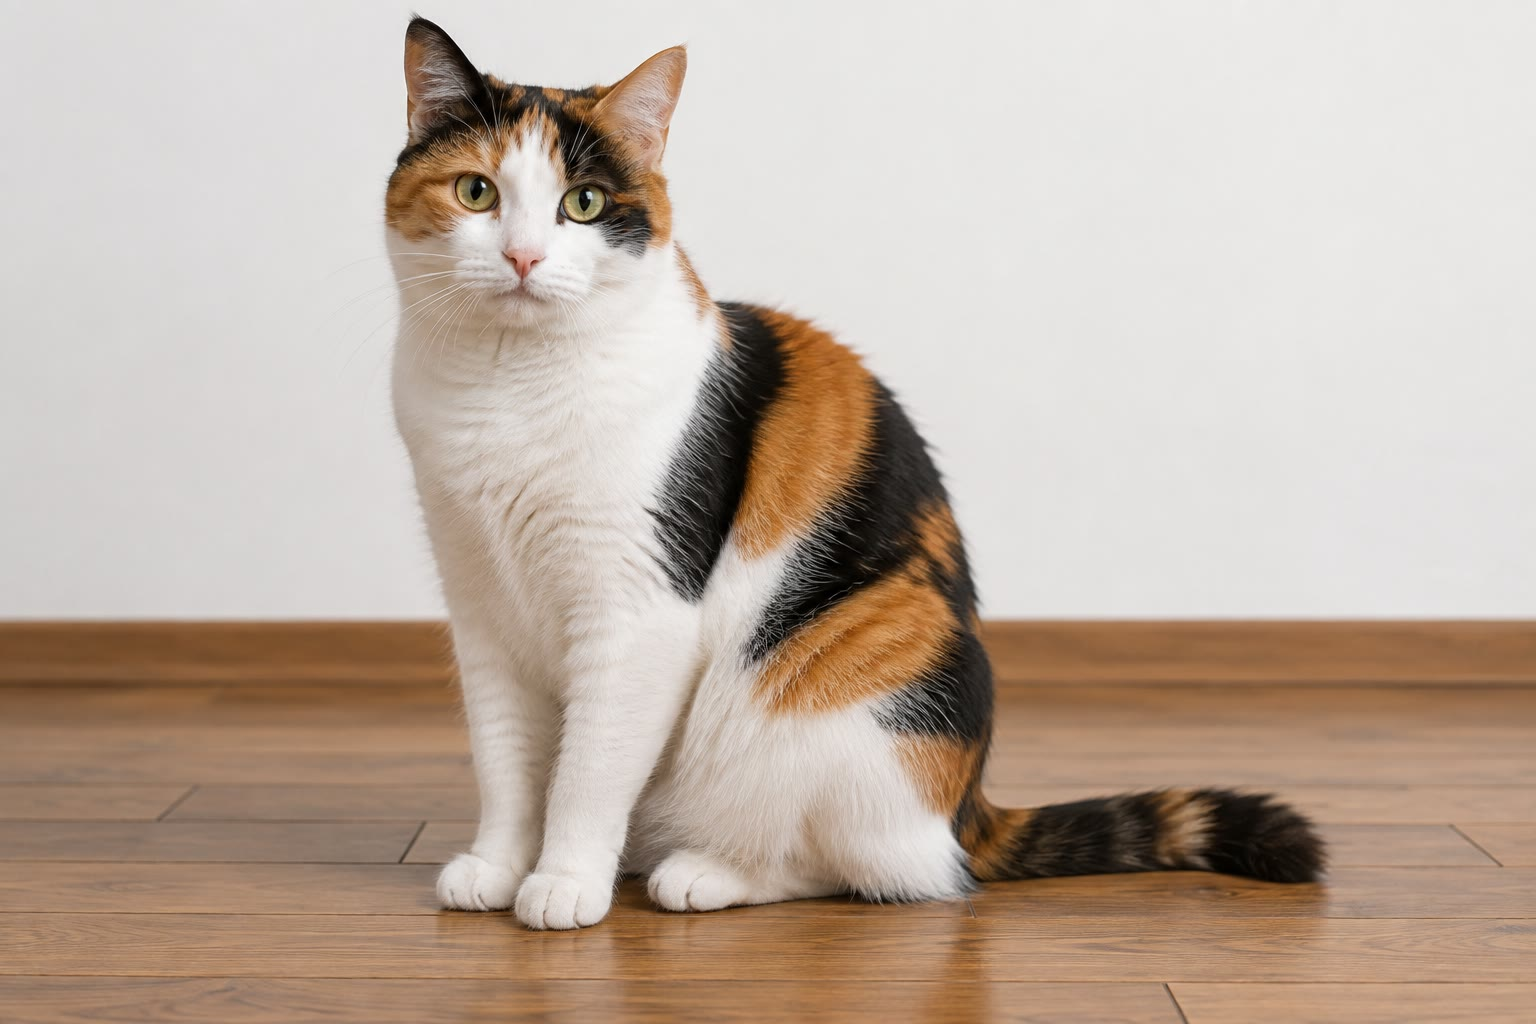
\includegraphics[width=0.5\linewidth]{images/book5/ai/b5-01-calico-cat.jpg}

{\small Kiri: nukleus sel betina yang diwarnai untuk DNA, dengan X tak aktif
yang mampat --- \omterm{def:b3:chromatin-epigenetics:x-inactivation}{badan Barr} --- terhimpit pada tepi intinya. Kanan: seekor
kucing belang tiga. Tiap bercak jingga atau hitam adalah satu klon sel kulit
yang membungkam kromosom X yang sama; warna putihnya berasal dari gen
pembercak autosom yang terpisah.}
\end{omfigure}

\begin{definition}[Pencetakan genomik]\label{def:b3:chromatin-epigenetics:imprinting}
\index{pencetakan genomik}\index{daerah kendali pencetakan}\index{disomi uniparental}
Sebuah gen disebut \emph{tercetak} apabila hanya satu dari kedua alelnya yang
diekspresikan, dan alel mana yang diekspresikan bergantung pada tetua asalnya:
sebagian gen hanya diekspresikan dari salinan ayah, sebagian lain hanya dari
salinan ibu. Mamalia memiliki sekitar \numrange{100}{200} gen tercetak yang
mengelompok, dan tiap kelompok dikendalikan oleh sebuah \emph{daerah kendali
pencetakan} (ICR) yang termetilasi pada satu alel tetua dan tidak pada yang
lain. Metilasinya dipasang di dalam garis nutfah --- satu pola di dalam
sperma, pola lain di dalam telur --- dihapus di dalam sel nutfah generasi
berikutnya lalu dipasang lagi menurut jenis kelamin individu tersebut. Anak
yang menerima kedua salinan sebuah kromosom dari tetua yang sama
(\emph{disomi uniparental}) karena itu memiliki dosis gen tercetak yang salah
walaupun urutannya sama sekali normal.
\end{definition}

\begin{proof}[Bukti eksperimental]
McGrath dan Solter, dan secara terpisah Surani, Barton, serta Norris (1984),
membuat zigot mencit berpronukleus dua-duanya dari ibu, atau dua-duanya dari
ayah, dengan memindahkan pronukleus antartelur yang telah dibuahi. Kedua
macam zigot itu tidak berkembang sampai lahir, walaupun masing-masing
memiliki dua perangkat kromosom yang lengkap: embrio ginogenetiknya membentuk
embrio yang lumayan dengan plasenta yang buruk, sedangkan yang androgenetik
membentuk plasenta besar dan nyaris tanpa embrio. Kedua genom tetua itu tidak
setara dan keduanya diperlukan. Cattanach dan Kirk (1985) menunjukkan dengan
\omterm{def:b3:chromatin-epigenetics:imprinting}{disomi uniparental} khas-kromosom bahwa ketaksetaraan itu terbatas pada daerah
tertentu kromosom tertentu, dan di situlah kelompok gen tercetak kemudian
ditemukan.
\end{proof}

\begin{example}[Kelompok \emph{Igf2}--\emph{H19}]\label{ex:b3:chromatin-epigenetics:igf2}
\emph{Igf2}, sebuah faktor pertumbuhan janin, diekspresikan dari alel ayah;
tetangganya \emph{H19}, sebuah RNA tak penyandi, dari alel ibu. Di antara
keduanya terletak ICR dan, di seberang \emph{H19}, seperangkat penguat
bersama. Pada kromosom dari ibu, ICR-nya tak termetilasi dan mengikat CTCF,
yang bertindak sebagai isolator: penguatnya dapat menjangkau \emph{H19}
tetapi tidak \emph{Igf2}. Pada kromosom dari ayah, ICR-nya termetilasi
(dipasang di dalam sperma), CTCF tidak dapat mengikat, dan penguatnya
menjangkau ke seberang sampai \emph{Igf2}; metilasinya juga merambat sehingga
membungkam promotor \emph{H19}. Satu tanda, dipasang di satu garis nutfah,
memutuskan nasib kedua gen.
\end{example}

\begin{omfigure}
\begin{tikzpicture}[every node/.style={font=\scriptsize}, >=stealth]
  \foreach \yy/\lab/\ctcf in {1.6/kromosom dari ibu/1, -0.6/kromosom dari ayah/0} {
    \draw[very thick, gray] (0,\yy) -- (9.4,\yy);
    \node[left, align=right] at (-0.15,\yy) {\lab};
    \draw[thick, fill=omDef!25] (1.0,\yy-0.2) rectangle (2.6,\yy+0.2); \node at (1.8,\yy) {\emph{Igf2}};
    \draw[thick, fill=omProp!30] (4.2,\yy-0.2) rectangle (5.2,\yy+0.2); \node at (4.7,\yy) {ICR};
    \draw[thick, fill=omDef!25] (6.2,\yy-0.2) rectangle (7.4,\yy+0.2); \node at (6.8,\yy) {\emph{H19}};
    \foreach \x in {8.4,8.8,9.2} \fill[omMeth!70!black] (\x,\yy) circle (0.12);
    \node[right] at (9.55,\yy) {penguat};
  }
  % maternal: CTCF bound, enhancer -> H19
  \draw[thick, fill=omExo!35] (4.7,2.15) ellipse (0.45 and 0.22); \node at (4.7,2.15) {CTCF};
  \draw[->, thick, omMeth!70!black] (8.4,1.85) .. controls (7.8,2.5) and (7.2,2.5) .. (6.8,1.85);
  \node[above] at (7.6,2.35) {aktif};
  \draw[thick, omThm] (5.3,2.3) -- (5.3,0.9); \node[omThm, below] at (5.3,0.9) {isolator};
  \node[omThm, above=1.0cm, align=center, font=\scriptsize] at (1.8,1.8) {\emph{Igf2} bisu};
  % paternal: ICR methylated
  \foreach \x in {4.35,4.6,4.85,5.1} \fill[omThm] (\x,-0.95) circle (0.08);
  \node[below, align=center] at (4.7,-1.05) {termetilasi:\\tanpa CTCF};
  \draw[->, thick, omMeth!70!black] (8.4,-0.35) .. controls (6.5,0.6) and (3.5,0.6) .. (1.8,-0.35);
  \node[above] at (3.3,0.2) {aktif};
  \foreach \x in {6.4,6.7,7.0,7.2} \fill[omThm] (\x,-0.95) circle (0.08);
  \node[below] at (6.8,-1.05) {dibungkam};
\end{tikzpicture}

{\small Pencetakan pada \emph{Igf2}--\emph{H19}. Alel dari ibu: ICR yang tak
termetilasi mengikat CTCF, sebuah isolator, sehingga penguat di hilirnya
hanya mengaktifkan \emph{H19}. Alel dari ayah: ICR-nya termetilasi di dalam
sperma, CTCF tidak dapat mengikat, penguatnya menjangkau \emph{Igf2}, dan
metilasinya membungkam \emph{H19}.}
\end{omfigure}

\begin{example}[Prader--Willi dan Angelman]\label{ex:b3:chromatin-epigenetics:pws}
Penghapusan yang sama sebesar kira-kira \qty{5}{Mb} pada kromosom 15 (daerah
15q11--q13) menimbulkan \emph{sindrom Prader--Willi} --- tonus otot yang
lemah saat lahir, lalu nafsu makan tak terpuaskan dan kegemukan --- apabila
penghapusan itu berada pada kromosom dari ayah, dan \emph{sindrom Angelman}
--- disabilitas intelektual berat, tanpa bicara, perangai riang, dan
kejang --- apabila berada pada kromosom dari ibu. Daerah itu mengusung gen
yang diekspresikan dari ayah (\emph{SNRPN} dan sekelompok RNA kecil) yang
satu-satunya salinan aktifnya hilang pada kasus pertama, dan \emph{UBE3A}
yang diekspresikan dari ibu, yang hilang pada kasus kedua. \omterm{def:b3:chromatin-epigenetics:imprinting}{Disomi uniparental}
ibu untuk kromosom 15, tanpa penghapusan sama sekali, juga memberi
Prader--Willi: dua salinan dari ibu, bisu untuk gen dari ayah.
\end{example}

\begin{remark}[Mengapa mencetak sama sekali]\label{rem:b3:chromatin-epigenetics:kinship}
Gen tercetak diperkaya untuk kendali pertumbuhan janin dan pemindahan hara
plasenta, dengan gen yang diekspresikan dari ayah (\emph{Igf2}, \emph{Peg3})
cenderung memacu pertumbuhan dan gen yang diekspresikan dari ibu
(\emph{H19}, \emph{Igf2r}, \emph{Cdkn1c}) cenderung mengekangnya. Yang
disebut \emph{teori kekerabatan} membaca hal ini sebagai pertentangan: gen
seorang ayah beruntung bila menyedot lebih banyak dari ibu yang kelak mungkin
mengandung keturunan jantan lain, sedangkan gen ibu beruntung bila menjatah
di antara seluruh anaknya. Pencetakan terjadi pada mamalia berplasenta dan
pada tumbuhan berbunga, yang endospermanya juga disuapi induknya, dan tidak
pada burung maupun reptil --- persis seperti ramalan teori itu.
\end{remark}

\section{Pewarisan epigenetik dan batasnya}

\begin{definition}[Epigenetika]\label{def:b3:chromatin-epigenetics:epigenetics}
\index{epigenetika}\index{epialel}\index{pemrograman ulang}
Yang disebut \emph{epigenetika} adalah kajian tentang perubahan aktivitas gen
yang diwariskan tanpa berupa perubahan urutan DNA: keadaan yang diusung oleh
\omterm{def:b3:chromatin-epigenetics:methylation}{metilasi DNA}, tanda \omterm{def:b3:chromatin-epigenetics:nucleosome}{histon}, atau untaian faktor transkripsi yang menopang
dirinya sendiri, lalu disalin lewat pembelahan sel. Dua alel yang urutannya
identik tetapi keadaan epigenetiknya berbeda dan mantap disebut
\emph{epialel}. Pewarisan lewat mitosis adalah kelaziman dan itulah yang
membuat sel terdiferensiasi tetap terdiferensiasi. Pewarisan lewat meiosis,
dari tetua ke keturunan, merupakan kekecualian pada mamalia, karena tandanya
dihapus dalam dua gelombang \emph{pemrograman ulang}: di dalam sel nutfah
purba, tempat cetakan dan sebagian besar metilasi disapu lalu dipasang
kembali menurut jenis kelaminnya, dan sekali lagi di dalam zigot serta embrio
dini, tempat genom dari ayah didemetilasi secara aktif oleh TET3 dan genom
dari ibu secara pasif, sebelum pola embrio itu sendiri diletakkan oleh DNMT3.
\end{definition}

\begin{example}[Mencit kuning agouti yang bertahan hidup]\label{ex:b3:chromatin-epigenetics:agouti}
Pada alel $A^{vy}$ sebuah retrotransposon menyisip di hulu gen warna bulu
\emph{agouti}. Di tempat promotor transposon itu tak termetilasi, promotor
tersebut memacu \emph{agouti} terus-menerus di setiap sel; mencitnya kuning,
gemuk, dan rawan diabetes. Di tempat promotor itu termetilasi, gennya
mengikuti kendali normalnya dan mencitnya cokelat (``pseudoagouti''). Saudara
seperindukan yang identik secara genetik terentang di sepanjang seluruh
spektrum itu, dan induk kuning beranak kuning lebih banyak daripada induk
cokelat: \omterm{def:b3:chromatin-epigenetics:epigenetics}{epialelnya} terhapus secara tidak tuntas lewat garis nutfah ibu.
Waterland dan Jirtle (2003) memberi induk $A^{vy}$ yang bunting pakan kaya
pendonor metil (folat, vitamin B\textsubscript{12}, kolina, betaina) dan
menggeser bulu anaknya ke arah cokelat. Lingkungan satu generasi telah
memasang tanda yang diusung generasi berikutnya.
\end{example}

\begin{omfigure}
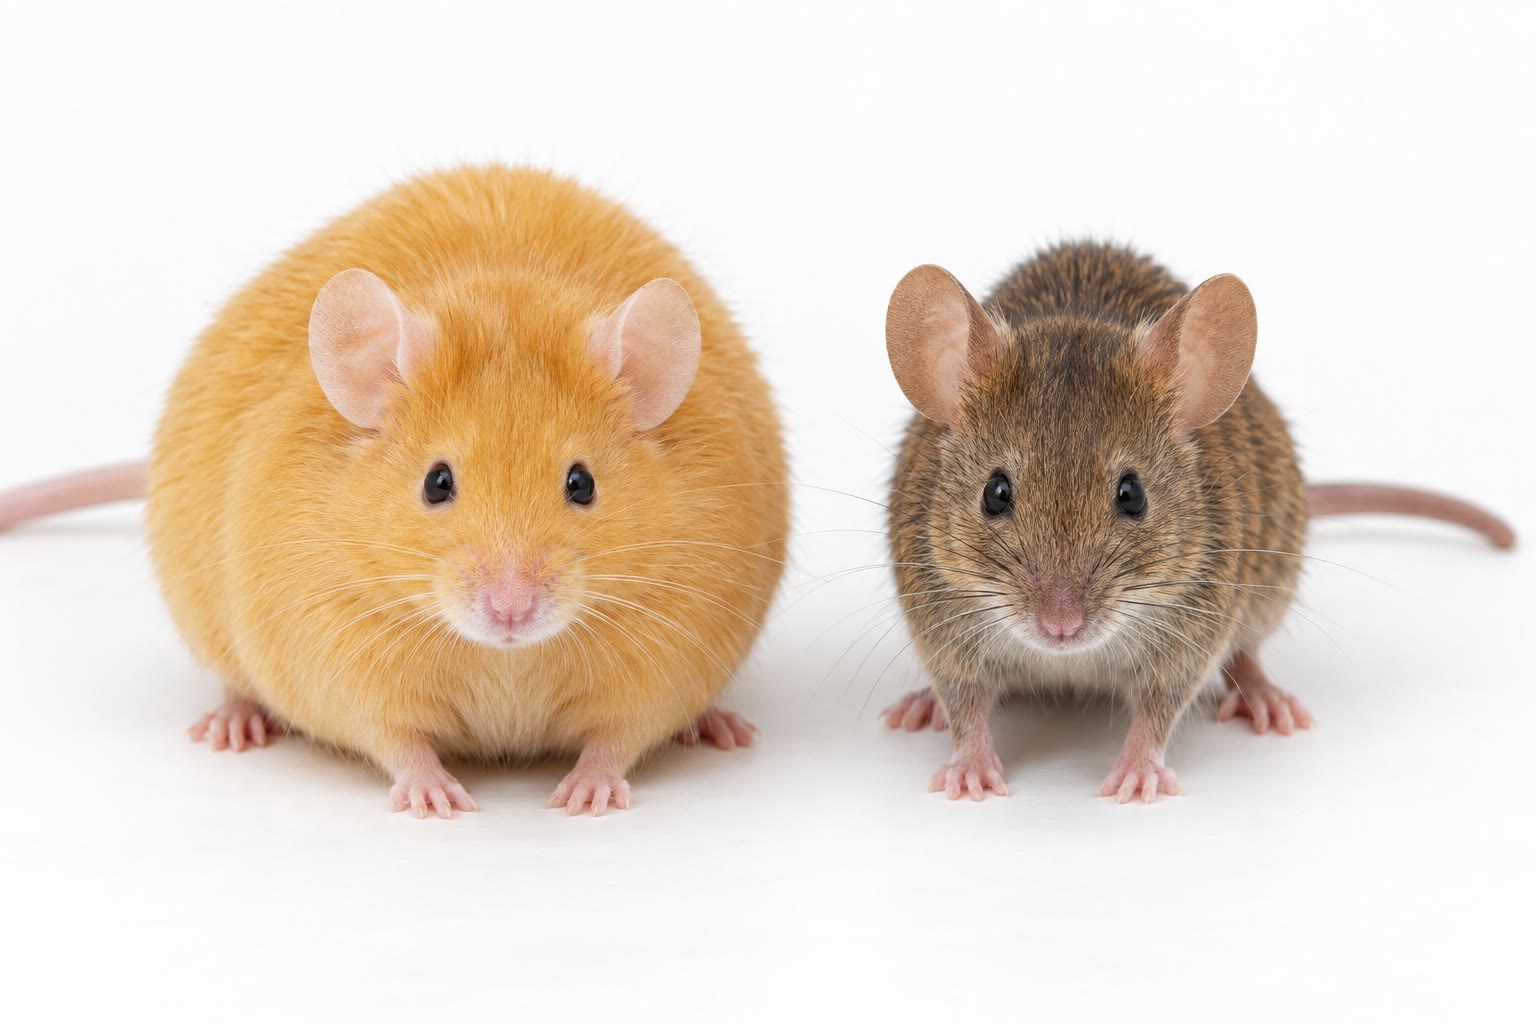
\includegraphics[width=0.62\linewidth]{images/book5/ai/b5-01-agouti-mice.jpg}

{\small Dua saudara seperindukan $A^{vy}$ dengan genotipe identik: seekor
mencit kuning dan gemuk yang transposon di hulu \emph{agouti}-nya tak
termetilasi, dan seekor pseudoagouti cokelat yang transposon itu termetilasi.}
\end{omfigure}

\begin{proposition}[Di mana keadaan epigenetik yang diwariskan ditemukan]\label{prop:b3:chromatin-epigenetics:examples}
\index{variegasi efek posisi}\index{vernalisasi}\index{paramutasi}
Tiga sistem yang telah dianalisis dengan baik memperagakan mekanisme di atas.
\emph{\omterm{prop:b3:chromatin-epigenetics:examples}{Variegasi efek posisi}} pada \emph{Drosophila}: sebuah gen yang
dipindahkan oleh penataan ulang kromosom sehingga berdampingan dengan
\omterm{def:b3:chromatin-epigenetics:nucleosome}{heterokromatin} dibungkam pada sebagian sel dan tidak pada sebagian lain,
sehingga matanya belang; tiap bercak adalah satu klon, pembungkamannya
merambat dari \omterm{def:b3:chromatin-epigenetics:nucleosome}{heterokromatin} lewat gelung HP1, dan gen yang mutasinya menekan
variegasi itu (gen \emph{Su(var)}) ternyata HP1 dan metiltransferase H3K9.
\emph{Vernalisasi} pada \emph{Arabidopsis}: dingin musim dingin selama
berminggu-minggu membungkam penekan pembungaan \emph{FLC} lewat H3K27me3 yang
diletakkan Polycomb, kebisuan itu bertahan sepanjang berbulan-bulan
pertumbuhan musim semi dan ribuan pembelahan sel, dan keadaannya diatur ulang
pada tiap generasi sehingga tiap tumbuhan harus mengalami musim dinginnya
sendiri. \emph{Paramutasi} pada jagung: satu alel gen pigmen \emph{b1},
ketika berjumpa dengan alel tertentu yang lain di dalam heterozigot,
mengubahnya menjadi keadaan bisu miliknya sendiri, dan alel yang telah
berubah itu meneruskan keadaannya kepada keturunannya selama berbagai
generasi, lewat metilasi terarah-RNA-kecil yang dibahas di
\cref{ch:b3:rna-regulation}. Pada tiap kasus pewarisannya bersifat mitotik
dan tangguh; penerusan antargenerasinya entah diatur ulang secara aktif
(tumbuhan) atau bocor dan sebagian (mencit).
\end{proposition}

\begin{remark}[Batas klaim antargenerasi]\label{rem:b3:chromatin-epigenetics:limits}
Klaim bahwa kelaparan atau tekanan batin seorang kakek ``diwariskan secara
epigenetik'' kepada cucu manusia sering terdengar dan sebagian besar belum
terbukti. Dua gelombang penghapusan berdiri di antara sebuah tanda somatik
dan seorang cucu, gen tercetak serta segelintir transposon adalah satu-satunya
penyintas penghapusan yang terdokumentasi pada mamalia, dan di dalam kohort
manusia pengaruh lingkungan bersama, lingkungan rahim, serta selisih genetik
sukar dipisahkan dari sebuah tanda yang diusung garis nutfah. Kasus yang
telah diperagakan --- $A^{vy}$, sebagian \omterm{def:b3:chromatin-epigenetics:epigenetics}{epialel} terpaut transposon, keadaan
yang diperantarai RNA pada cacing dan tumbuhan --- memang nyata, dipahami
secara molekuler, dan sempit. Teorema bab ini menjelaskan sebabnya: tanpa
umpan balik yang mendorong $\mu$ ke $1$, sebuah tanda melupakan dirinya dalam
beberapa lusin pembelahan, dan garis nutfah menambahkan pengaturan ulang yang
aktif di atasnya.
\end{remark}

\section{Latihan}

\begin{exercise}[$\star$]\label{exo:b3:chromatin-epigenetics:1}
Sebutkanlah susunan partikel inti sebuah \omterm{def:b3:chromatin-epigenetics:nucleosome}{nukleosom}, panjang DNA yang
diikatnya, dan panjang penghubung yang lazim. Mengapa pencernaan \omterm{def:b3:chromatin-epigenetics:nucleosome}{kromatin}
dengan nuklease memberi tangga fragmen, bukan lapisan merata?
\end{exercise}

\begin{exercise}[$\star$]\label{exo:b3:chromatin-epigenetics:2}
Sebuah genom katak memiliki $3.0\times 10^{9}$ pasangan basa tiap perangkat
haploid. Berapa \omterm{def:b3:chromatin-epigenetics:nucleosome}{nukleosom} yang dikandung sebuah nukleus diploid, dengan
ulangan \qty{190}{bp}, dan berapa panjang DNA-nya?
\end{exercise}

\begin{exercise}[$\star$]\label{exo:b3:chromatin-epigenetics:3}
Uraikanlah H3K27me3, H4K16ac, dan H3S10ph. Untuk masing-masing katakan apakah
ia berkaitan dengan \omterm{def:b3:chromatin-epigenetics:nucleosome}{kromatin} aktif atau bisu, lalu sebutkan satu \omterm{def:b3:chromatin-epigenetics:histone-code}{pembaca} bagi
yang pertama.
\end{exercise}

\begin{exercise}[$\star$]\label{exo:b3:chromatin-epigenetics:4}
Jelaskanlah mengapa kucing belang tiga hampir selalu betina, dan apa yang
pasti dimiliki kucing belang tiga jantan.
\end{exercise}

\begin{exercise}[$\star\star$]\label{exo:b3:chromatin-epigenetics:5}
Hitunglah \omterm{prop:b3:chromatin-epigenetics:compaction}{rasio pemampatan} serabut \qty{10}{nm} dari angka-angka
\cref{def:b3:chromatin-epigenetics:nucleosome} (ulangan \qty{200}{bp},
manik \qty{11}{nm}), dan rasio yang dibutuhkan untuk memuat \qty{4}{cm} DNA
kromosom manusia rata-rata ke dalam kromatid mitosis sepanjang
\qty{4}{\micro m}. Dengan faktor tambahan berapa serabut itu harus terlipat?
\end{exercise}

\begin{exercise}[$\star\star$]\label{exo:b3:chromatin-epigenetics:6}
Di dalam model \cref{thm:b3:chromatin-epigenetics:maintenance} dengan
$\mu = 0.98$ dan $\delta = 0.01$, carilah $p^{*}$ dan cacah pembelahan yang
membuat tapak yang mula-mula termetilasi kehilangan separuh kelebihannya
atas $p^{*}$. Ulangilah untuk $\mu = 0.999$, $\delta = 0.001$.
\end{exercise}

\begin{exercise}[$\star\star$]\label{exo:b3:chromatin-epigenetics:7}
Sebuah percobaan ChIP-seq pada sel hati memberi puncak H3K4me3 dan puncak
H3K27ac pada promotor gen $A$, domain H3K27me3 yang lebar di atas gen $B$,
dan H3K9me3 di atas gen $C$. Ramalkanlah keadaan transkripsi masing-masing,
lalu katakan mana di antara $B$ dan $C$ yang lebih mungkin menyala pada tipe
sel lain, dan mengapa.
\end{exercise}

\begin{exercise}[$\star\star$]\label{exo:b3:chromatin-epigenetics:8}
Seorang perempuan membawa penghapusan daerah \emph{UBE3A} pada salah satu
kromosom 15-nya tetapi sehat. Ayahnya membawa penghapusan yang sama dan juga
sehat. Sindrom apa, bila ada, yang mengancam tiap anaknya, dan dengan peluang
berapa? Bagaimana andaikan penghapusan itu datang dari ibunya?
\end{exercise}

\begin{exercise}[$\star\star$]\label{exo:b3:chromatin-epigenetics:9}
Ramalkanlah akibatnya, pada embrio mencit betina, apabila gen
\emph{\omterm{def:b3:chromatin-epigenetics:x-inactivation}{Xist}} dihapus dari satu kromosom X; dari keduanya. Ramalkanlah apa yang
dilakukan transgen \emph{\omterm{def:b3:chromatin-epigenetics:x-inactivation}{Xist}} yang disisipkan ke sebuah autosom pada autosom itu.
\end{exercise}

\begin{exercise}[$\star\star\star$]\label{exo:b3:chromatin-epigenetics:10}
Jelaskanlah, dengan \cref{ex:b3:chromatin-epigenetics:cpg-deficit}, mengapa
\omterm{def:b3:chromatin-epigenetics:methylation}{pulau CpG} mempertahankan \omterm{def:b3:chromatin-epigenetics:methylation}{CpG-nya} sedangkan sisa genom kehilangan empat
perlimanya, dan apa yang tersirat dari hal itu tentang keadaan metilasi
pulau-pulau tersebut di dalam garis nutfah sepanjang waktu evolusi. Mengapa
argumen itu gagal bagi gen yang hanya termetilasi di dalam hati?
\end{exercise}

\begin{exercise}[$\star\star\star$]\label{exo:b3:chromatin-epigenetics:11}
Tunjukkanlah, dengan gelung penulis--pembaca
\cref{prop:b3:chromatin-epigenetics:readers}, bagaimana sebuah domain H3K9me3
dapat mantap sepanjang replikasi walaupun tiap pembelahan mengencerkan \omterm{def:b3:chromatin-epigenetics:nucleosome}{histon}
bertanda itu dua kali lipat dengan \omterm{def:b3:chromatin-epigenetics:nucleosome}{histon} baru tanpa tanda. Apa yang
menentukan tempat domain itu berhenti merambat? Usulkanlah percobaan untuk menguji uraian Anda.
\end{exercise}

\begin{exercise}[$\star\star\star$]\label{exo:b3:chromatin-epigenetics:12}
Sebuah kajian melaporkan bahwa cucu orang yang mengalami masa kelaparan
memiliki metilasi yang berubah pada sebuah gen pertumbuhan dan massa tubuh
yang lebih besar. Sebutkanlah penjelasan tandingan yang harus disingkirkan
sebelum menyimpulkan bahwa sebuah tanda metilasi diteruskan lewat garis
nutfah, lalu katakan percobaan apa pada mencit yang akan menuntaskan soal itu.
\end{exercise}

\section{Soal: Ingatan Sebuah Gen yang Dibungkam}

\begin{problem}[{Soal akhir pekan --- sebuah genom manusia yang terkemas ke
dalam nukleusnya, sebuah tanda metilasi yang diikuti sepanjang pembelahan,
seekor kucing belang tiga yang dibaca sebagai peta klonal, dan penyakit satu
daerah tercetak yang dihitung, berakhir pada cacah pembelahan yang dilalui
sebuah tanda tanpa umpan balik dan pada ukuran populasi sel yang memilih X-nya}]
\label{pb:b3:chromatin-epigenetics:1}
Data: sebuah nukleus diploid manusia memuat $6.4\times 10^{9}$ pasangan basa,
pada \qty{0.34}{nm} dan \qty{650}{Da} tiap pasangan; ulangan \omterm{def:b3:chromatin-epigenetics:nucleosome}{nukleosomnya}
\qty{200}{bp}, sebuah oktamer \omterm{def:b3:chromatin-epigenetics:nucleosome}{histon} berbobot \qty{108}{kDa}, dan partikel
intinya berupa cakram bergaris tengah \qty{11}{nm} dan setebal \qty{5.5}{nm}.
Nukleusnya bola bergaris tengah \qty{10}{\micro m}. Genomnya
\qty{42}{\%} G$+$C. Metilasi pada \omterm{def:b3:chromatin-epigenetics:methylation}{CpG} biasa: $\mu = 0.99$,
$\delta = 0.02$ tiap pembelahan.

\medskip
\noindent\textbf{Bagian I --- Pengemasan.}
\begin{enumerate}
  \item Hitunglah panjang total DNA di dalam nukleus dan cacah
        \omterm{def:b3:chromatin-epigenetics:nucleosome}{nukleosomnya}.
  \item Hitunglah massa total \omterm{def:b3:chromatin-epigenetics:nucleosome}{histon} (oktamernya saja) dan massa DNA,
        dalam pikogram ($\qty{1}{Da} = \qty{1.66e-24}{g}$).
  \item Hitunglah volume nukleus dan volume total partikel intinya, yang
        diperlakukan sebagai silinder. Berapa bagian nukleus yang
        diisinya?
  \item Andaikan \omterm{def:b3:chromatin-epigenetics:nucleosome}{nukleosomnya} dijajarkan ujung ke ujung sebagai serabut
        \qty{10}{nm}, berapa panjang serabut itu, dan berapa \omterm{prop:b3:chromatin-epigenetics:compaction}{rasio
        pemampatannya} terhadap DNA telanjang?
  \item Serabut itu terlipat menjadi simpal sepanjang \qty{200}{kb} yang
        tertambat kohesin. Berapa simpal, dan berapa \omterm{def:b3:chromatin-epigenetics:nucleosome}{nukleosom} tiap simpal?
  \item Dengan andaian kebebasan, berapa dinukleotida \omterm{def:b3:chromatin-epigenetics:methylation}{CpG} yang akan
        dikandung genom diploid itu? Cacah teramatinya
        $5.6\times 10^{7}$. Berapa bagian yang hilang, dan lewat
        mekanisme mutasi apa?
\end{enumerate}

\medskip
\noindent\textbf{Bagian II --- Sebuah tanda sepanjang pembelahan.}
\begin{enumerate}[resume]
  \item Tulislah rekurensi bagi $p_{n}$ lalu hitunglah $p^{*}$.
  \item Sebuah \omterm{def:b3:chromatin-epigenetics:methylation}{CpG} promotor termetilasi penuh pada $n = 0$. Hitunglah $p_{n}$
        sesudah $10$, $50$, dan $200$ pembelahan.
  \item Sesudah berapa pembelahan kelebihan $p_{n} - p^{*}$ tinggal separuh?
        Sel punca jaringan membelah kira-kira sekali seminggu: berapa tahun
        lamanya itu?
  \item Sebuah obat menghambat \omterm{def:b3:chromatin-epigenetics:methylation}{DNMT1} sepenuhnya ($\mu = 0$) dan DNMT3 juga
        ($\delta = 0$). Tunjukkanlah bahwa fraksi untai termetilasi di dalam
        populasinya separuh pada tiap pembelahan, lalu carilah cacah
        pembelahan yang membawa metilasi \qty{80}{\%} ke bawah \qty{5}{\%}.
  \item Di dalam pulau yang dibungkam, \omterm{def:b3:chromatin-epigenetics:histone-code}{pembaca} \omterm{def:b3:chromatin-epigenetics:methylation}{metil-CpG} merekrut metilasi
        H3K9, yang merekrut DNMT3, sehingga di dalam pulau itu
        $\mu = 0.9995$ dan $\delta = 0.0005$. Hitunglah ulang waktu paruh
        kelebihannya, dalam pembelahan dan dalam tahun pada satu pembelahan
        seminggu.
  \item Jelaskanlah dalam satu kalimat mengapa hasil pertanyaan 11 dan bukan
        hasil pertanyaan 9 yang dituntut sebuah gen yang dibungkam seumur
        hidup, dan susunan molekul macam apa yang menghasilkannya.
\end{enumerate}

\medskip
\noindent\textbf{Bagian III --- Peta belang tiga.}
\begin{enumerate}[resume]
  \item Seekor kucing heterozigot untuk gen jingga terpaut-X. Jelaskanlah
        mengapa bulunya berbercak jingga dan hitam dan apa yang diwakili
        satu bercak.
  \item \omterm{def:b3:chromatin-epigenetics:x-inactivation}{Penonaktifan X} terjadi ketika sel yang ditakdirkan membentuk kulit
        berjumlah $N$. Masing-masing memilih X secara acak. Berapa peluang
        bahwa seluruh $N$ sel memilih X yang sama, sehingga kucingnya
        berwarna tunggal?
  \item Tidak ada heterozigot berwarna tunggal semacam itu yang
        terdokumentasi di antara barangkali semiliar ekor kucing; ambillah
        peluangnya sebesar $10^{-9}$ lalu taksirlah $N$.
  \item Luas permukaan kulit kucing itu sekitar \qty{0.3}{m^2} dan
        bercaknya rata-rata \qty{15}{cm^2}. Taksirlah cacah bercaknya, lalu
        jelaskan mengapa cacah itu lebih besar daripada $N$.
  \item Seekor kucing jantan XXY juga belang tiga. Berapa \omterm{def:b3:chromatin-epigenetics:x-inactivation}{badan Barr} yang
        tampak pada selnya? Berapa pada betina XXX dan pada jantan XY?
  \item Sebuah gen yang lolos dari penonaktifan hadir dalam dua salinan
        aktif pada betina dan satu pada jantan. Berikanlah satu alasan
        mengapa pelolosan itu dapat ditoleransi dan satu keadaan tempat hal
        itu penting.
\end{enumerate}

\medskip
\noindent\textbf{Bagian IV --- Kromosom 15.}
\begin{enumerate}[resume]
  \item Sindrom Prader--Willi mengenai kira-kira satu kelahiran dari
        \num{15000}; \qty{70}{\%} kasusnya berupa penghapusan de novo
        15q11--q13 dari ayah dan \qty{25}{\%} berupa \omterm{def:b3:chromatin-epigenetics:imprinting}{disomi uniparental}
        ibu. Hitunglah frekuensi kelahiran tiap sebabnya.
  \item Sindrom Angelman berfrekuensi kira-kira sama; \qty{70}{\%} berupa
        penghapusan dari ibu, \qty{5}{\%} disomi dari ayah, dan
        \qty{10}{\%} mutasi titik \emph{UBE3A}. Mengapa mutasi titik
        menjadi sebab Angelman tetapi hampir tak pernah menjadi sebab
        Prader--Willi?
  \item Seorang ayah membawa translokasi berimbang yang membuat
        \qty{20}{\%} spermanya kehilangan 15q11--q13. Berapa bagian anaknya
        yang mengidap Prader--Willi, dan berapa bagian yang Angelman?
  \item \omterm{def:b3:chromatin-epigenetics:imprinting}{Disomi uniparental} timbul ketika zigot trisomik kehilangan satu
        kromosom. Bila zigot trisomi-15 kehilangan satu dari ketiga
        kromosomnya secara acak, dan trisominya berasal dari ibu (dua
        salinan dari ibu), berapa peluang bahwa yang tersisa berupa disomi
        ibu? Sindrom yang mana?
  \item Gen Prader--Willi diekspresikan dari ayah dan gen Angelman dari
        ibu. Dengan teori kekerabatan, katakanlah gejala mana dari kedua
        sindrom itu (kesulitan menyusu saat lahir lawan nafsu makan yang
        rakus) yang cocok dengan teori tersebut dan mana yang lebih sukar
        dicocokkan.
  \item Diusulkan sebuah cara mengobati Angelman dengan mengaktifkan
        kembali \emph{UBE3A} dari ayah yang bisu. Kebisuannya disebabkan
        oleh RNA antisens yang diekspresikan dari ayah. Usulkanlah sasaran
        molekulnya lalu katakan mengapa terapi itu tidak akan mengganggu
        gen tercetak yang lain.
  \item Ringkaskanlah: waktu paruh sebuah tanda tanpa umpan balik
        (pertanyaan~9) dan dengan umpan balik (pertanyaan~11), dalam
        pembelahan; dan populasi pendiri $N$ bulu belang tiga
        (pertanyaan~15).
\end{enumerate}
\end{problem}
